\chapter{\textbf{Prosess og metode}}
\newthought I dette kapittelet skal vi gjøre rede for og drøfte vår prosjektplanlegging og arbeidsprosess

\subsection{\textbf{Historie}}

Software-utvikling er fortsatt en relativt ny bransje, mens prosjektstyring har  og det å styre et IT-prosjekt har vært. Det har vært stor diskusjon og utprøvning av en rekke prosjekt styringsformer. I dette avsnittet legger vi frem tre populære prosjektstyrings-metodikker samt diskuterer deres bruk.


\subsection{\textbf{Waterfall-metodikken}}

Waterfall er det første forsøket på en SDLC(Software development lifecycle) model. En SDLC er en prosess brukt i software utviklings industrien til å designe, utvikle og teste høy kvalitet software. En waterfall modell er veldig enkel å følge, nettopp fordi den er trinnbasert og visuelt ligner den på et fossefall. 

\begin{figure}[H] 
    \centering
    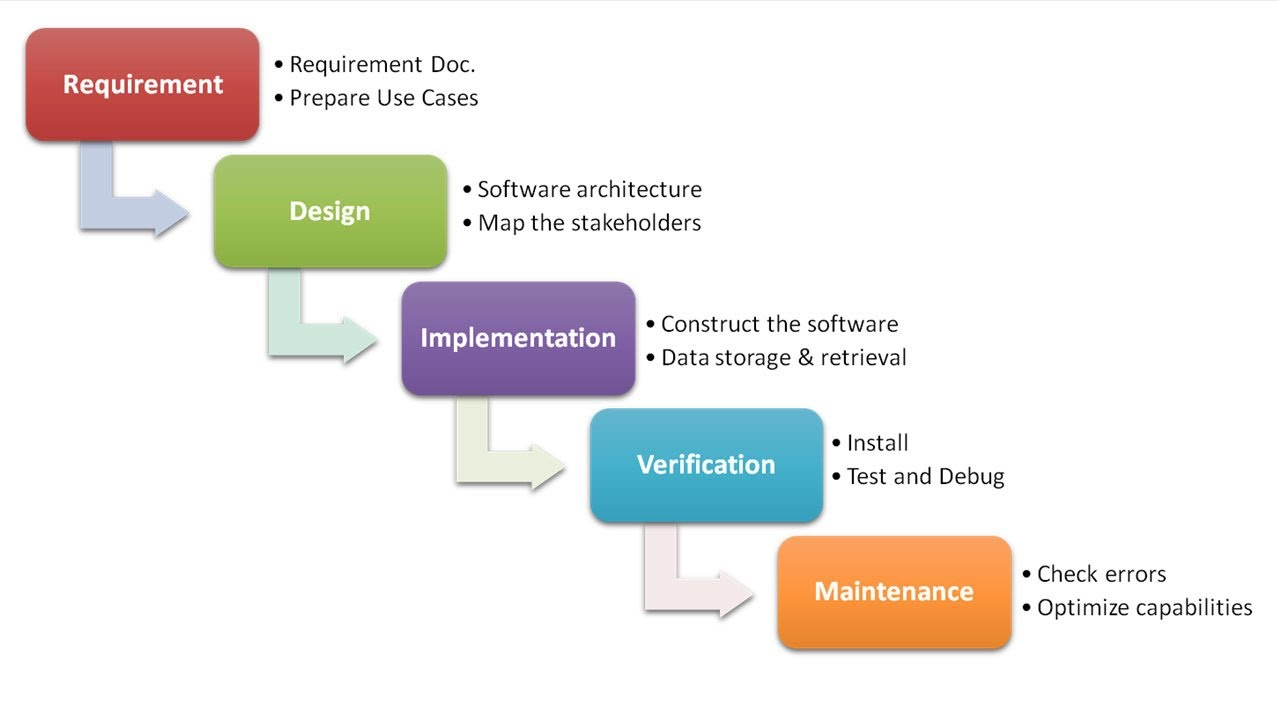
\includegraphics[width=\textwidth]{figures/Prosess-og-metode/waterfall.jpg}
    \caption{Waterfall}
\end{figure}



\paragraph{\textbf{Fordeler og ulemper med Waterfall}}

\textbf{Klar struktur}

Waterfall-metodikken skiller seg i stor grad fra de andre prosjektstyrings-metodikker ved at her "må" hvert trinn være gjennomført før arbeid på neste trinn starter. Denne lineære sekvensielle flyten står i sterk strid med nyere utviklingsmodeller, som for eksempel Agile/SCRUM. Dette gjørt at om det oppstår problemer så må disse håndteres med en gang for å ikke stoppe opp arbeidet. 

\textbf{Krystallklart sluttresultat}

Tidlig i prosessen defineres sluttresultatet. Dette fungerer godt for prosjekter hvor


\subsection{Agile}











